\section{Final-state Coulomb repulsion}
The effects of final-state Coulomb repulsion may be estimated by numerically solving the classical equations of motion of the $3\alpha$ system subject only to the Coulomb force from a fixed distance and outwards, see e.g.\ Refs.~\cite{norbeck68,thompson72}. Given the positions, $\boldsymbol{x}_i(t)\,$, and the momenta, $\boldsymbol{p}_i(t)\,$, of the three $\alpha$ particles at a given time, $t$, we compute the positions and momenta at time $t+\Delta t$ as 
\begin{align}\label{eq : coulomb numerical}
\boldsymbol{p}_i(t+\Delta t) &= \boldsymbol{p}_i(t) + \boldsymbol{F}_i(\boldsymbol{x}_1,\boldsymbol{x}_2,\boldsymbol{x}_3) \, \Delta t \nonumber \; , \\
\boldsymbol{x}_i(t+\Delta t) &= \boldsymbol{x}_i(t) + \frac{\boldsymbol{p}_i(t+\Delta t)}{m_{\alpha}} \, \Delta t \; .
\end{align}
Here, $\boldsymbol{F}_i(\boldsymbol{x}_1,\boldsymbol{x}_2,\boldsymbol{x}_3)$ is the Coulomb force on the $i^{\textrm{th}}$ $\alpha$ particle, and $\Delta t=10^{-25}$~s is the chosen time step. Energy conservation is used to check the numerical precision. 

We initiate the computation at $t=0$ with the primary $\alpha$ particle ($\alpha_1$) separated by a distance, $d_{1}$, from the center of mass of the two secondary $\alpha$ particles ($\alpha_2$, $\alpha_3$) which are 
separated from one another by a distance $d_{23}=4.5$~fm. The 
three-body energy is $\sum_{i\in\{1,2,3\}} E_{i} = 16.62-7.27 = 9.35$~MeV. 
Computations are performed for several values of the two-body 
energy $E_{23} = 2.0$, 3.0, 4.0, 5.0, 6.0~MeV and different relative orientations of the primary and secondary breakups, $\theta_2 = 5^{\circ}, 15^{\circ}, \dots, 85^{\circ}$. %
At $t=0$, the energy so far liberated in the form of kinetic energy to $\alpha_1$ and the recoiling $^8$Be nucleus is $\sum_{i\in\{1,2,3\}} E_{i} - E_{23} - V_{\textrm{C}}\,$, where $V_{\textrm{C}}$ is the Coulomb energy of the initial $3\alpha$ configuration. Using Eq.~\ref{eq : coulomb numerical}, we calculate the evolution the $3\alpha$ system out to several thousand~fm where the Coulomb repulsion becomes negligible. Finally, we compute the Dalitz coordinates $x = \sqrt{3} (E_2 - E_3) / \sum_{i} E_{i}$ and $y = (2 E_1 - E_2 - E_3) / \sum_{i} E_{i}$. 

The results of two such sets of computations, performed assuming initial separations of $d_{1}=10$~fm and 15~fm, are shown in Fig~\ref{fig:coulomb}. The arrows indicate the displacement of the Dalitz coordinates $x$, $y$ resulting from the final-state Coulomb repulsion. As expected, the computations assuming the closer initial separation of 10~fm and the larger two-body energy of $E_{23}=6.0$~MeV produce the largest displacements. Moreover, we observe that the largest displacements occur at the periphery of the Dalitz plot, i.e., for co-axial emission.  
We note that the chosen separations are consistent with naive expectations based on the known lifetime of the $^8$Be resonance and classical estimates of the relative velocities of the breakup fragments. 

\begin{figure}[htpb]
	\centering
	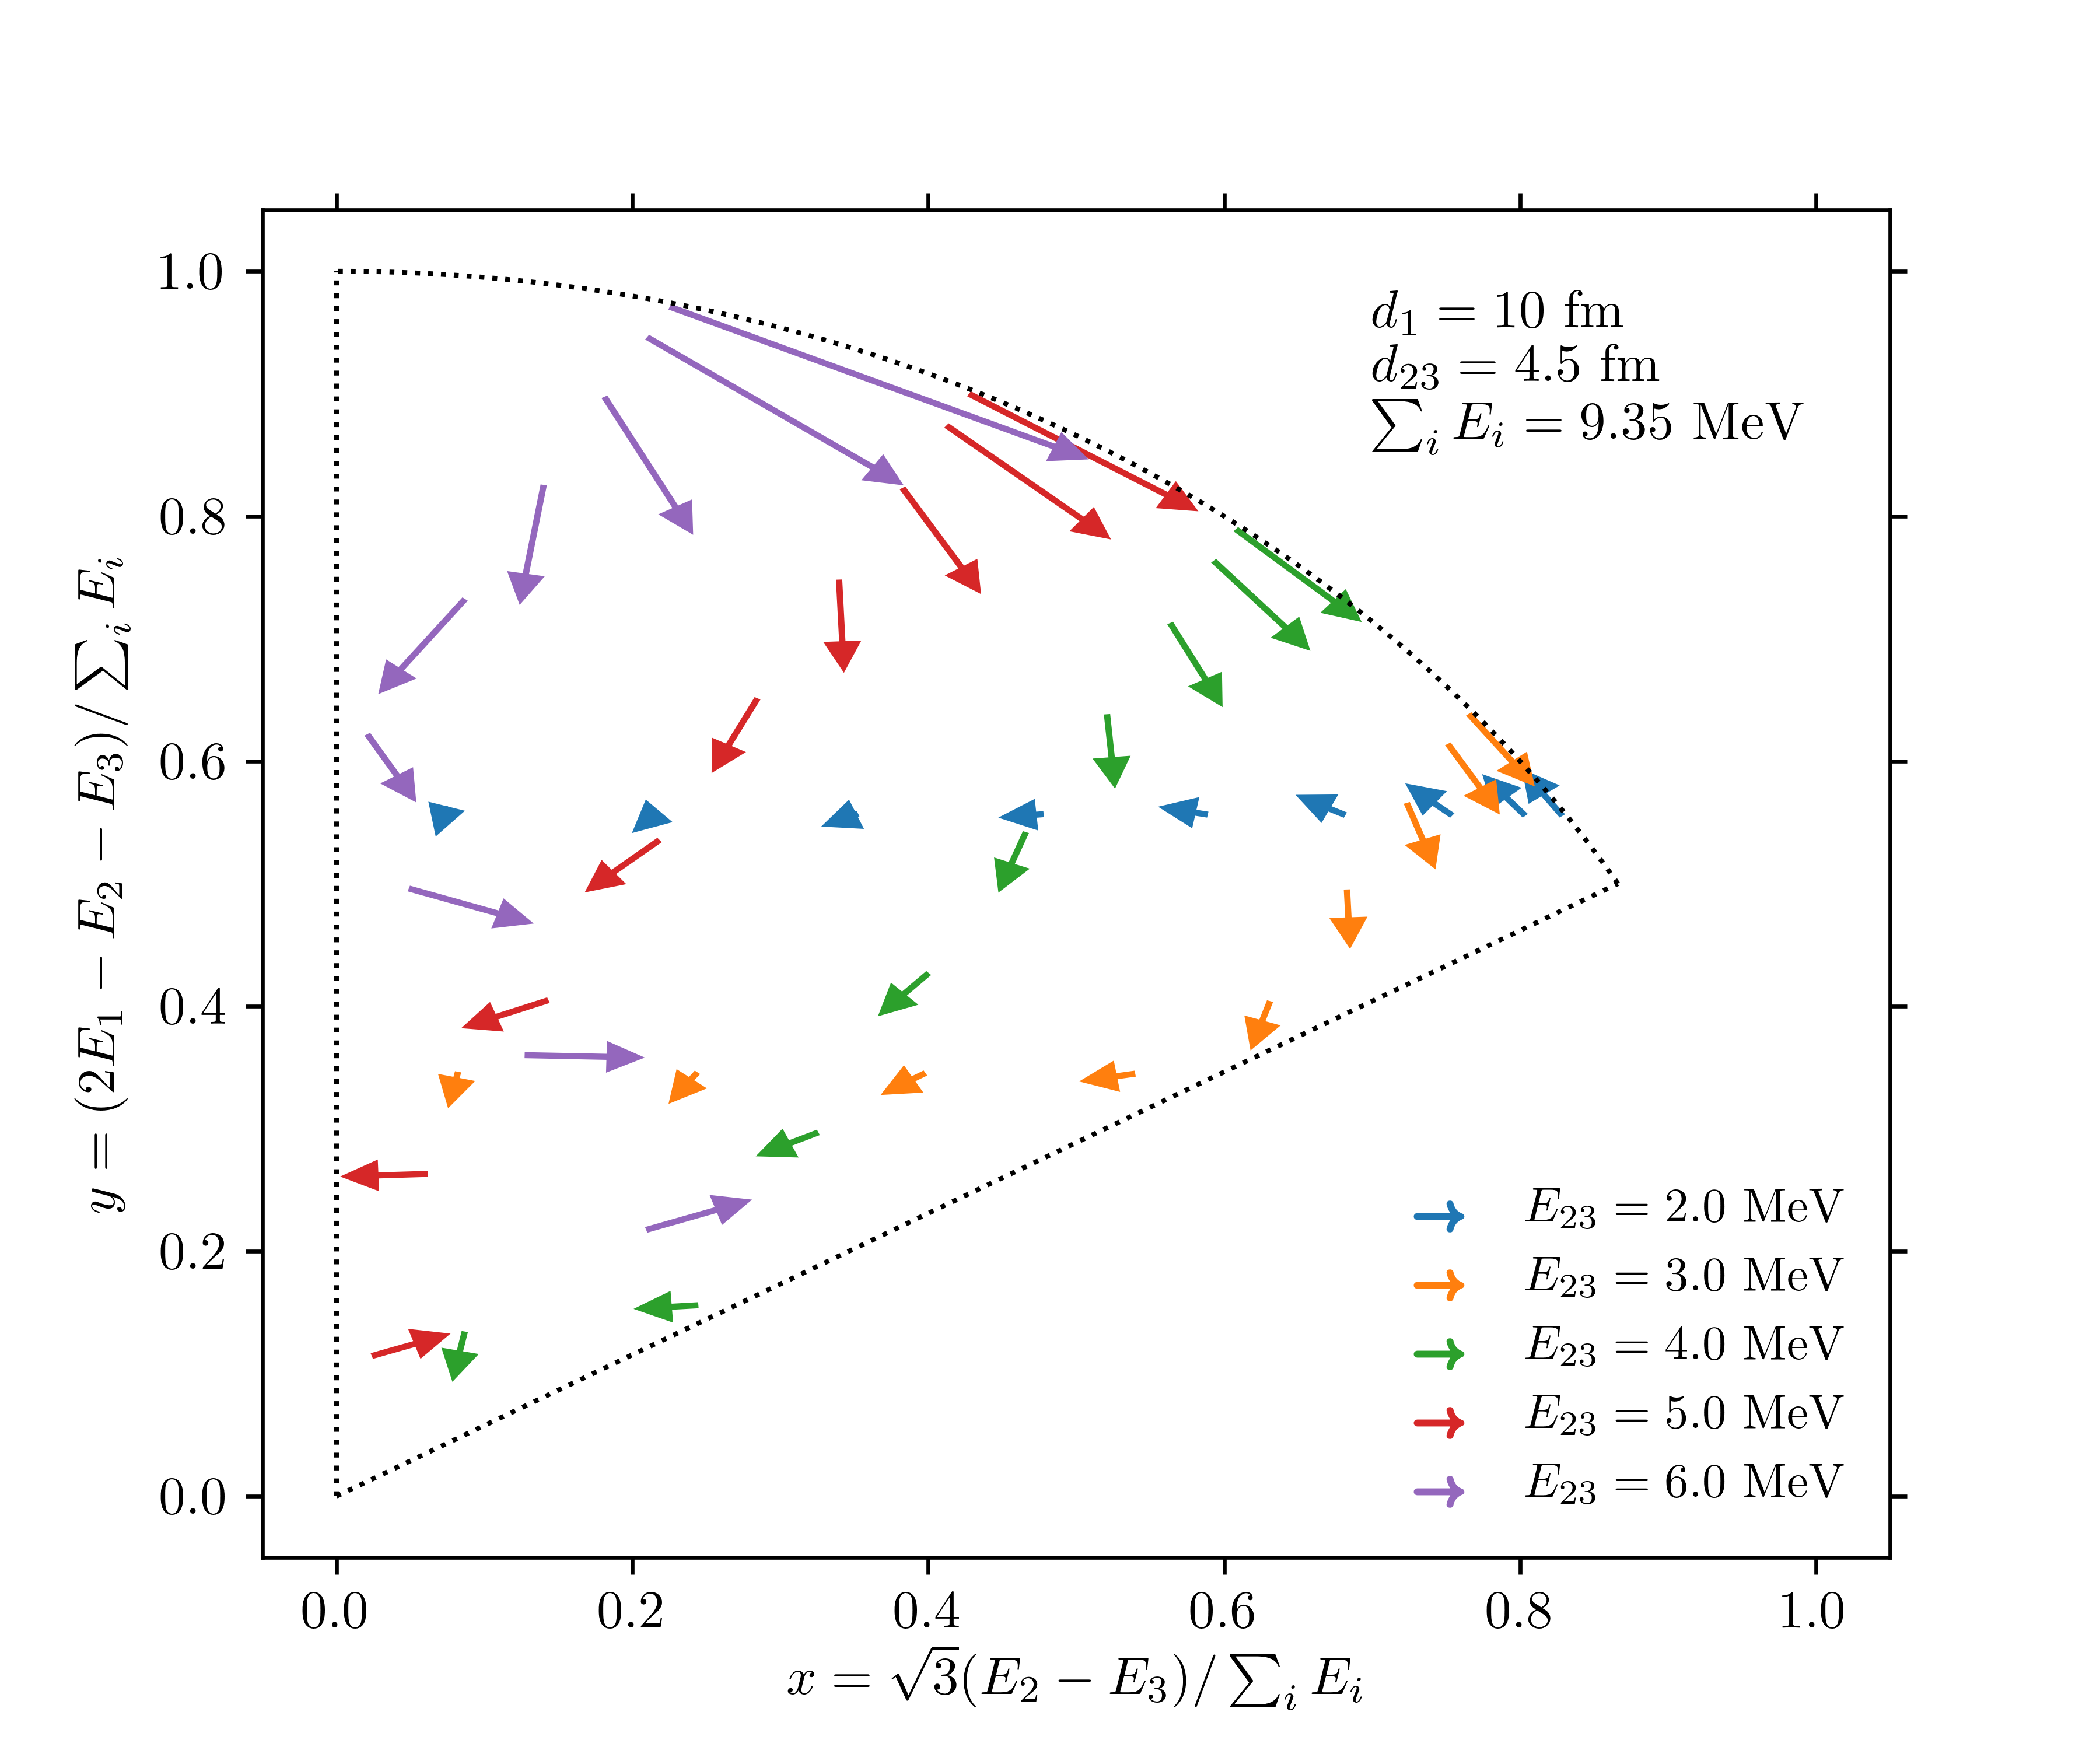
\includegraphics[width=0.9\linewidth]{coul3a_10fm_pretty.pdf}
	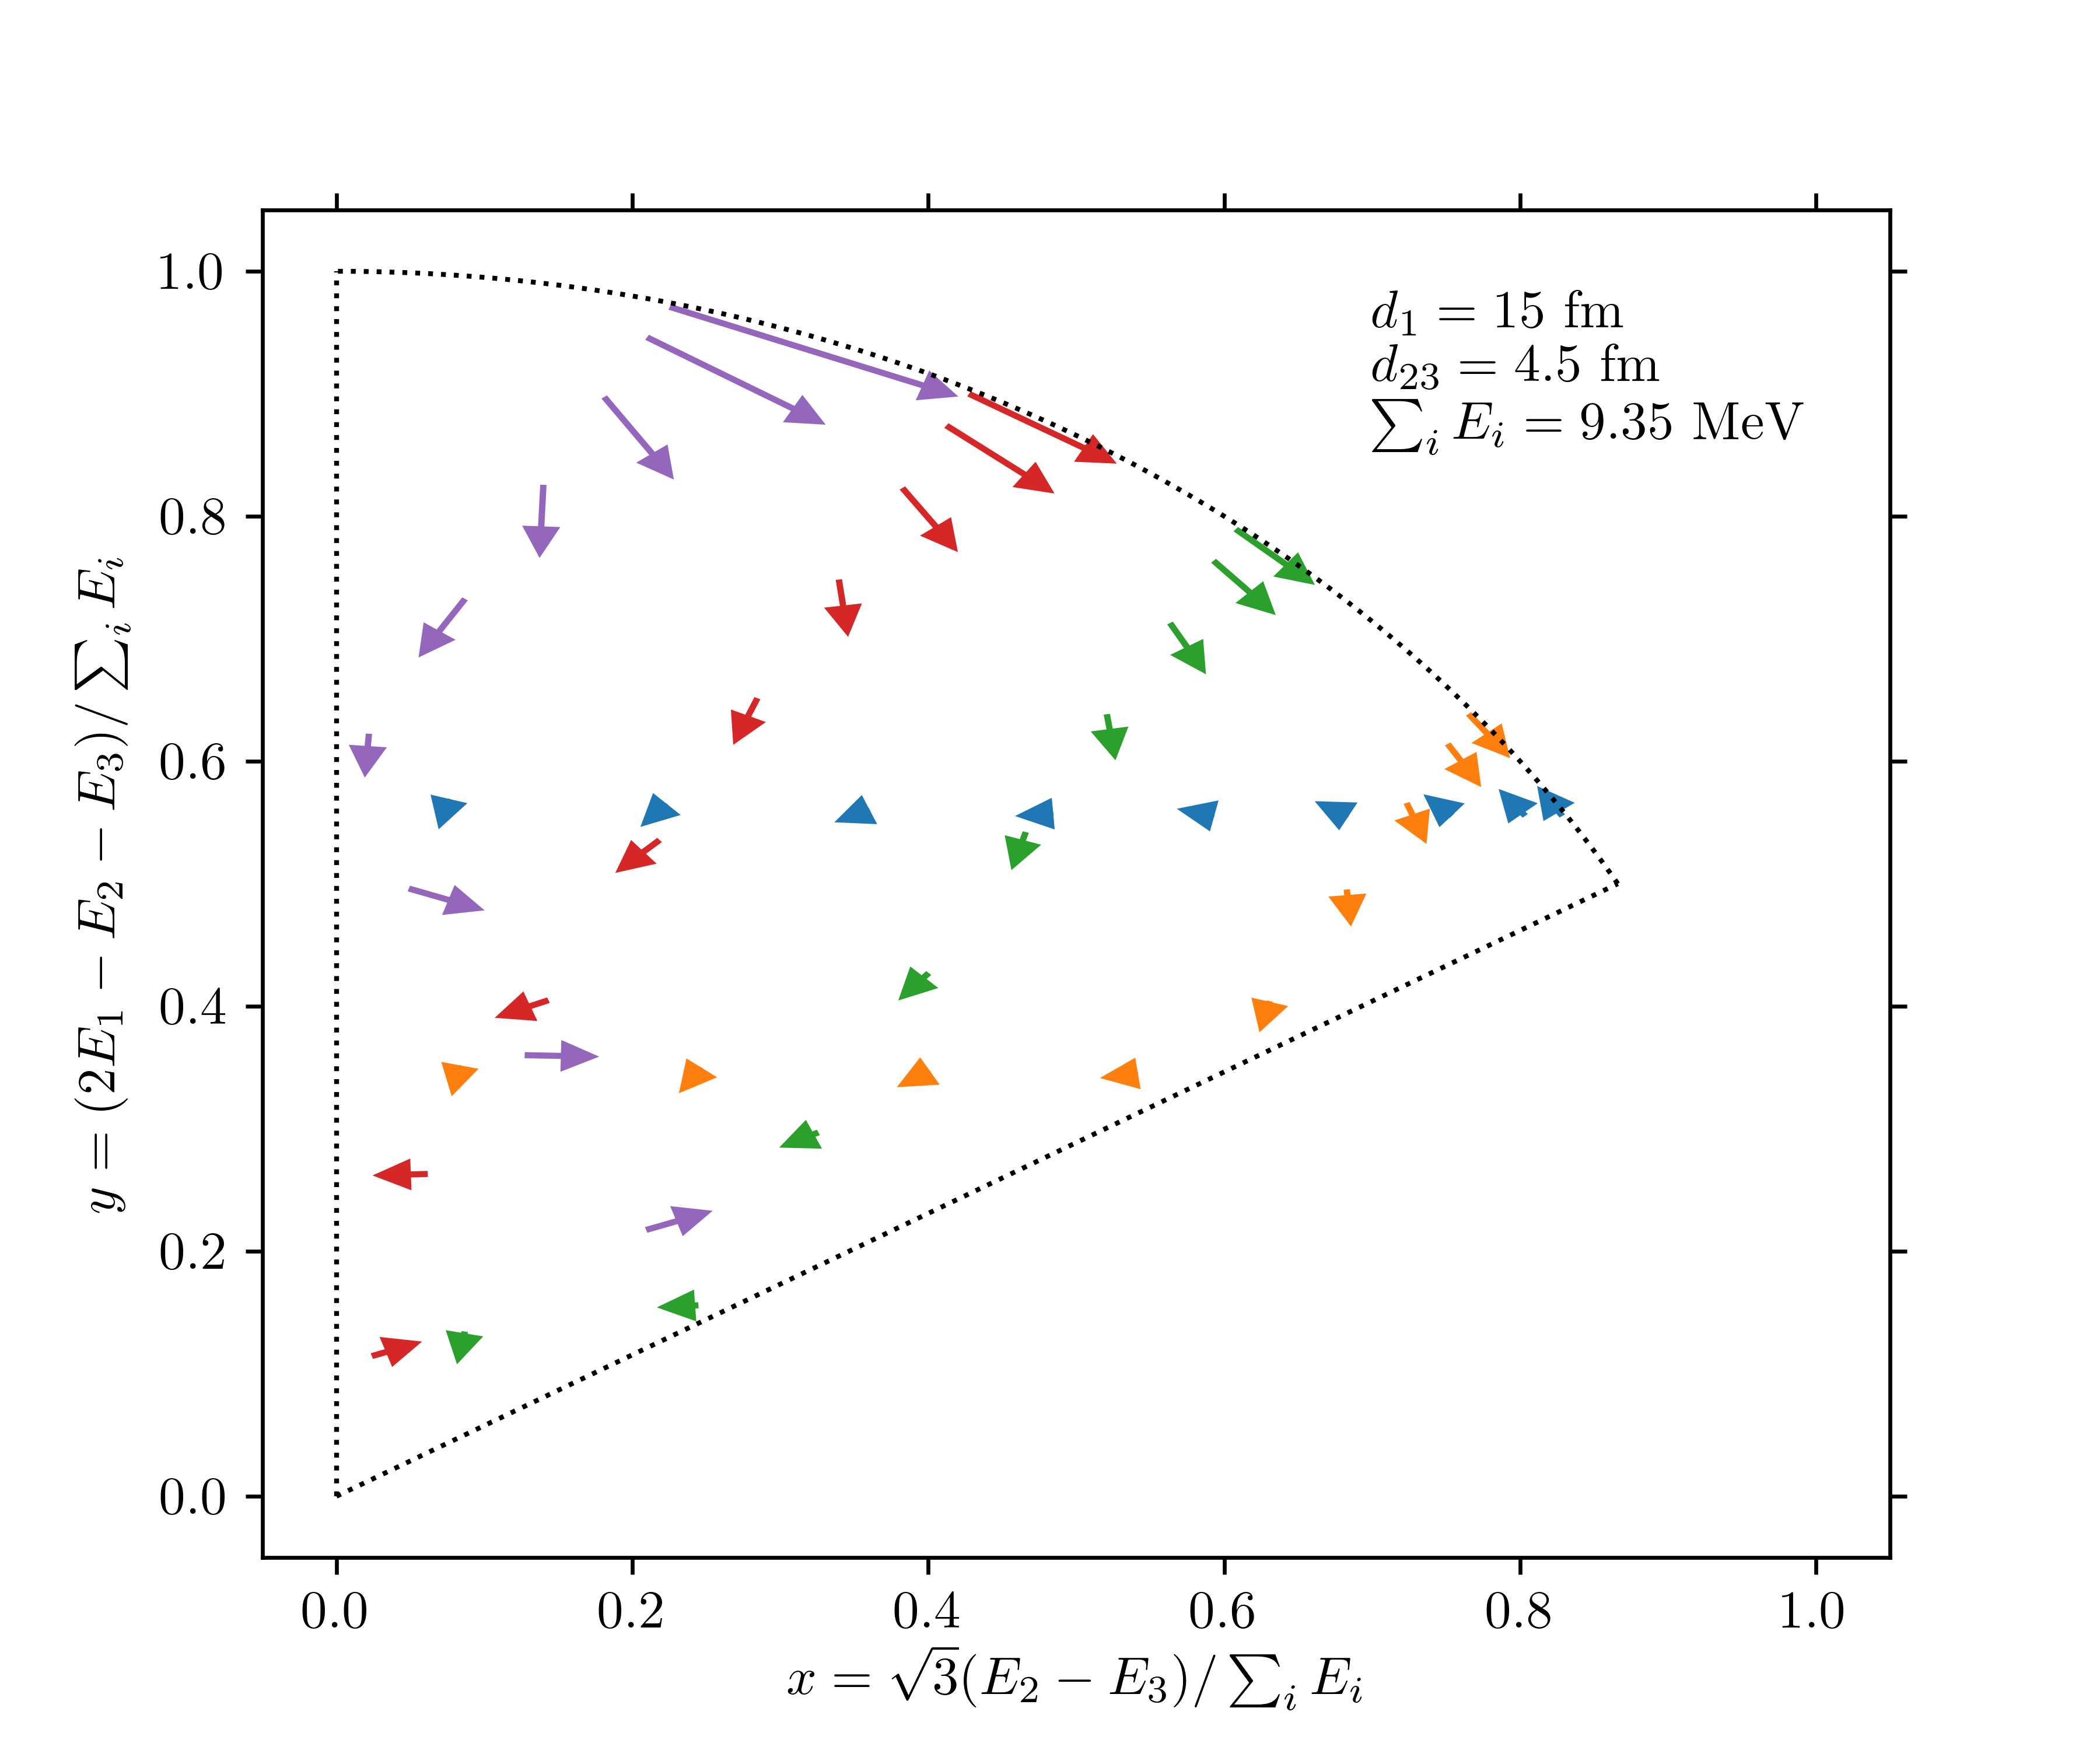
\includegraphics[width=0.9\linewidth]{coul3a_15fm_pretty.pdf}
	\caption{
		 Effects of final-state Coulomb repulsion estimated by numerically solving the classical equations of motion of the $3\alpha$ system, assuming initial separations of $d_{1}=10$~fm (top) and 15~fm (bottom). See text for details. The arrows indicate the displacement of the Dalitz coordinates $x$, $y$ resulting from the Coulomb repulsion.
	}
	\label{fig:coulomb}
\end{figure}
